\documentclass{article}
\usepackage[utf8]{inputenc}

\title{Homework 3 - Classification; Decision Tree; Ensemble Learning}
\author{Benny Chen}
\date{\today}

\usepackage{color}
\usepackage{amsthm}
\usepackage{amssymb} 
\usepackage{amsmath}
\usepackage{listings}
\usepackage{xcolor}
\usepackage{listings}
\usepackage{graphicx}
\usepackage[hidelinks]{hyperref}
\usepackage{enumitem}
\usepackage{tikz,forest}
\usetikzlibrary{arrows.meta}

\forestset{
    .style={
        for tree={
            base=bottom,
            child anchor=north,
            align=center,
            s sep+=1cm,
    straight edge/.style={
        edge path={\noexpand\path[\forestoption{edge},thick,-{Latex}] 
        (!u.parent anchor) -- (.child anchor);}
    },
    if n children={0}
        {tier=word, draw, thick, rectangle}
        {draw, diamond, thick, aspect=2},
    if n=1{%
        edge path={\noexpand\path[\forestoption{edge},thick,-{Latex}] 
        (!u.parent anchor) -| (.child anchor) node[pos=.2, above] {Y};}
        }{
        edge path={\noexpand\path[\forestoption{edge},thick,-{Latex}] 
        (!u.parent anchor) -| (.child anchor) node[pos=.2, above] {N};}
        }
        }
    }
}

\definecolor{codegreen}{rgb}{0,0.6,0}
\definecolor{codegray}{rgb}{0.5,0.5,0.5}
\definecolor{codepurple}{rgb}{0.58,0,0.82}
\definecolor{backcolour}{rgb}{0.95,0.95,0.92}

\lstdefinestyle{mystyle}{
    backgroundcolor=\color{backcolour},   
    commentstyle=\color{codegreen},
    keywordstyle=\color{magenta},
    numberstyle=\tiny\color{codegray},
    stringstyle=\color{codepurple},
    basicstyle=\ttfamily\footnotesize,
    breakatwhitespace=false,         
    breaklines=true,                 
    captionpos=b,                    
    keepspaces=true,                 
    numbers=left,                    
    numbersep=5pt,                  
    showspaces=false,                
    showstringspaces=false,
    showtabs=false,                  
    tabsize=2
}

\lstset{style=mystyle}

\begin{document}

\maketitle

\section{Classification and Decision Tree}

\subsection{General Knowledge about Decision Tree}

Consider a training set sampled uniformly from the the two-dimensional space shown in the following figure.

\begin{center}
    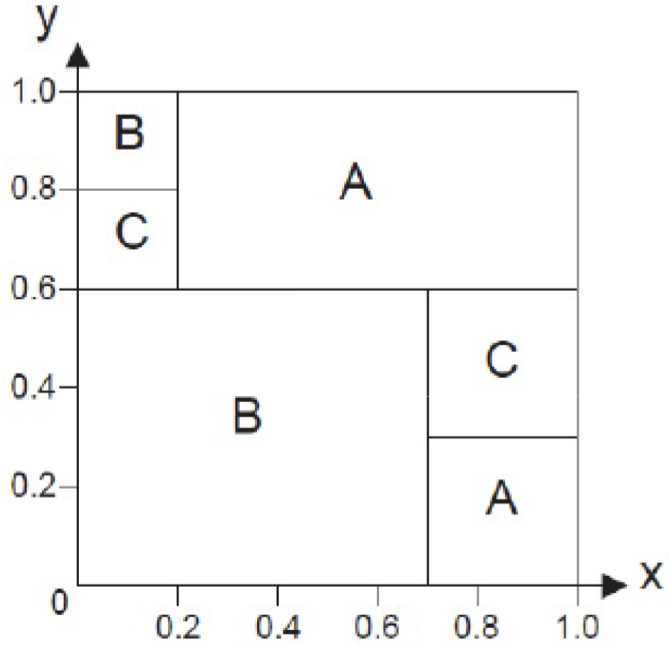
\includegraphics[scale=0.5]{images/q1.png}
\end{center}

The space is divided into three classes A, B, and C. Assume that the training set size is large enough so that the probabilities can be calculated accurately based on the areas of the selected regions (for instance, we can find the probability of sampling a data point of class B is p(B) = 0.42 + 0.04). You do not need to build a tree here,
but to calculate some essential entropy values to prepare a tree.

\begin{enumerate}[label=(\alph*)]
    \item Please compute the entropy for the overall data (considering that we have not decide any split point).
    \item If we split the data at $x \le 0.7$, what is the resulting entropy value?
\end{enumerate}

\begin{enumerate}[label=(\alph*)]
    \item We first calculate the areas of each class:
    \begin{equation}
        p(A) = (0.3 * 0.3) + (0.8 * 0.4) = 0.41
    \end{equation}
    \begin{equation}
        p(B) = (0.2 * 0.2) + (0.6 * 0.7) = 0.46
    \end{equation}
    \begin{equation}
        p(C) = (0.2 * 0.2) + (0.3 * 0.3) = 0.13
    \end{equation}

    We then calculate the entropy of each class:
    \begin{equation}
        -0.41 * log_2(0.41) - 0.46 * log_2(0.46) - 0.13 * log_2(0.13) = 1.425
    \end{equation}

    \item We first calculate the areas of each class:
    \begin{equation}
        p(A) = (0.5 * 0.4) = 0.2
    \end{equation}
    \begin{equation}
        p(B) = (0.2 * 0.2) + (0.6 * 0.7) = 0.46
    \end{equation}
    \begin{equation}
        p(C) = (0.2 * 0.2) = 0.04
    \end{equation}

    We then calculate the entropy of each class:
    \begin{equation}
        -0.2 * log_2(0.2) - 0.46 * log_2(0.46) - 0.04 * log_2(0.04) = 1.16
    \end{equation}

    We then multiply the entropy by the split which is 0.7:
    \begin{equation}
        0.7 * 1.16 = 0.812
    \end{equation}

    We also can calculate the entropy of the other half:
    \begin{equation}
        p(A) = (0.3 * 0.3) + (0.3 * 0.4) = 0.21
    \end{equation}
    \begin{equation}
        p(C) = (0.3 * 0.3) = 0.09
    \end{equation}

    We then calculate the entropy of each class:
    \begin{equation}
        -0.21 * log_2(0.21) - 0.09 * log_2(0.09) = 0.785
    \end{equation}

    We then multiply the entropy by the split which is 0.3:
    \begin{equation}
        0.3 * 0.785 = 0.235
    \end{equation}

    We then add the two entropy values together:
    \begin{equation}
        0.812 + 0.235 = 1.047
    \end{equation}

\end{enumerate}

\subsection{}

Suppose you are a player of THE LAST of US or imagine you are Joel or Ellie in this apocalypse. The following shows a history of a player in trying one episode of this game. We also indicate whether the episode is cleared or not in the last column. Note that the first column "ID" is for us to refer the record number only.

\begin{table}[h]
    \begin{tabular}{lllll}
    ID & Maximum Health & Stealth Skill & \begin{tabular}[c]{@{}l@{}}Listen Mode \\ Distance\end{tabular} & Clear the Episode \\
    1  & Enough         & Medium        & A                                                               & Yes               \\
    2  & High           & Medium        & A                                                               & Yes               \\
    3  & High           & Strong        & B                                                               & Yes               \\
    4  & High           & Strong        & C                                                               & Yes               \\
    5  & Few            & Medium        & B                                                               & No                \\
    6  & High           & Medium        & A                                                               & No                \\
    7  & Few            & Strong        & C                                                               & No                \\
    8  & Few            & Strong        & A                                                               & No               
    \end{tabular}
\end{table}

\begin{enumerate}[label=(\roman*)]
    \item Please find a C4.5 decision tree according to the above example. In the decision tree, whenever we process (1) a node containing at least 80\% records with the same label or (2) a node containing at most 2 records, we stop to process this node for splitting.
    \item Consider a trial with high maximum health, medium stealth skill, and A-level listen mode distance. Please estimate the probability that this trial will clear the episode.
\end{enumerate}

\begin{enumerate}[label=(\roman*)]
    \item 
    Entropy(Clear the Episode):
    \begin{equation}
        -\frac{1}{2}log_2(\frac{1}{2}) - \frac{1}{2}log_2(\frac{1}{2}) = 1
    \end{equation}
    Entropy(Maximum Health):
    \begin{equation}
        Entropy_{High} = -\frac{3}{4}log_2(\frac{3}{4}) - \frac{1}{4}log_2(\frac{1}{4}) = 0.811
    \end{equation}
    \begin{equation}
        Entropy_{Few} = -1log_2(1) = 0
    \end{equation}
    \begin{equation}
        Entropy_{Enough} = -1log_2(1) = 0
    \end{equation}
    Entropy(Clear the Episode | Maximum Health):
    \begin{equation}
        Entropy = \frac{4}{8}Entropy_{High} + \frac{3}{8}Entropy_{Few} + \frac{1}{8}Entropy_{Enough} = 0.405
    \end{equation}
    Split Information(Maximum Health):
    \begin{equation}
        SplitInfo = -\frac{4}{8}log_2(\frac{4}{8}) - \frac{3}{8}log_2(\frac{3}{8}) - \frac{1}{8}log_2(\frac{1}{8}) = 1.40563
    \end{equation}
    Gain(Maximum Health):
    \begin{equation}
        Gain = (1 - 0.405) / 1.40563 = 0.424
    \end{equation}
    Entropy(Stealth Skill):
    \begin{equation}
        Entropy_{Medium} = -\frac{2}{4}log_2(\frac{2}{4}) - \frac{2}{4}log_2(\frac{2}{4}) = 1
    \end{equation}
    \begin{equation}
        Entropy_{Strong} = -\frac{2}{4}log_2(\frac{2}{4}) - \frac{2}{4}log_2(\frac{2}{4}) = 1
    \end{equation}
    Entropy(Clear the Episode | Stealth Skill):
    \begin{equation}
        Entropy = \frac{4}{8}Entropy_{Medium} + \frac{4}{8}Entropy_{Strong} = 1
    \end{equation}
    Split Information(Stealth Skill):
    \begin{equation}
        SplitInfo = -\frac{4}{8}log_2(\frac{4}{8}) - \frac{4}{8}log_2(\frac{4}{8}) = 1
    \end{equation}
    Gain(Stealth Skill):
    \begin{equation}
        Gain = (1 - 1) / 1 = 0
    \end{equation}
    Entropy(Listen Mode Distance):
    \begin{equation}
        Entropy_{A} = -\frac{2}{4}log_2(\frac{2}{4}) - \frac{2}{4}log_2(\frac{2}{4}) = 1
    \end{equation}
    \begin{equation}
        Entropy_{B} = -\frac{1}{2}log_2(\frac{1}{2}) - \frac{1}{2}log_2(\frac{1}{2}) = 1
    \end{equation}
    \begin{equation}
        Entropy_{C} = -\frac{1}{2}log_2(\frac{1}{2}) - \frac{1}{2}log_2(\frac{1}{2}) = 1
    \end{equation}
    Entropy(Clear the Episode | Listen Mode Distance):
    \begin{equation}
        Entropy = \frac{4}{8}Entropy_{A} + \frac{2}{8}Entropy_{B} + \frac{2}{8}Entropy_{C} = 1
    \end{equation}
    Split Information(Listen Mode Distance):
    \begin{equation}
        SplitInfo = -\frac{4}{8}log_2(\frac{4}{8}) - \frac{2}{8}log_2(\frac{2}{8}) - \frac{2}{8}log_2(\frac{2}{8}) = 1.5
    \end{equation}
    Gain(Listen Mode Distance):
    \begin{equation}
        Gain = (1 - 1) / 1.5 = 0
    \end{equation}
    From the above calculation, we can see that the maximum gain is from Maximum Health, so we choose Maximum Health as the first node. We can now start creating the decision tree.

    \begin{forest}
        [Maximum Health
            [High
                [Yes 75\%]
                [No 25\%]
            ]
            [Enough
                [Yes 100\%]
                [No 0\%]
            ]
            [Few
                [Yes 0\%]
                [No 100\%]
            ]
        ]
    \centering
    \end{forest}

We now have to continue splitting the tree. We will use the same method as above to calculate the gain but this time only for Maximum Health = High data points so ID's 2,3,4, and 6.

Entropy(Clear the Episode):
\begin{equation}
    -\frac{3}{4}log_2(\frac{3}{4}) - \frac{1}{4}log_2(\frac{1}{4}) = 0.811
\end{equation}

Entropy(Stealth Skill):
\begin{equation}
    Entropy_{Medium} = -\frac{1}{2}log_2(\frac{1}{2}) - \frac{1}{2}log_2(\frac{1}{2}) = 1
\end{equation}
\begin{equation}
    Entropy_{Strong} = -1log_2(1) - 0log_2(0) = 0
\end{equation}
Entropy(Clear the Episode | Stealth Skill):
\begin{equation}
    Entropy = \frac{2}{4}Entropy_{Medium} + \frac{2}{4}Entropy_{Strong} = 0.5
\end{equation}
Split Information(Stealth Skill):
\begin{equation}
    SplitInfo = -\frac{2}{4}log_2(\frac{2}{4}) - \frac{2}{4}log_2(\frac{2}{4}) = 1
\end{equation}
Gain(Stealth Skill):
\begin{equation}
    Gain = (0.811 - 0.5) / 1 = 0.311
\end{equation}

Entropy(Listen Mode Distance):
\begin{equation}
    Entropy_{A} = -\frac{1}{2}log_2(\frac{1}{2}) - \frac{1}{2}log_2(\frac{1}{2}) = 1
\end{equation}
\begin{equation}
    Entropy_{B} = -1log_2(1) - 0log_2(0) = 0
\end{equation}
\begin{equation}
    Entropy_{C} = -1log_2(1) - 0log_2(0) = 0
\end{equation}
Entropy(Clear the Episode | Listen Mode Distance):
\begin{equation}
    Entropy = \frac{2}{4}Entropy_{A} + \frac{1}{4}Entropy_{B} + \frac{1}{4}Entropy_{C} = 0.5
\end{equation}
Split Information(Listen Mode Distance):
\begin{equation}
    SplitInfo = -\frac{2}{4}log_2(\frac{2}{4}) - \frac{1}{4}log_2(\frac{1}{4}) - \frac{1}{4}log_2(\frac{1}{4}) = 1.5
\end{equation}
Gain(Listen Mode Distance):
\begin{equation}
    Gain = (0.811 - 0.5) / 1.5 = 0.207
\end{equation}

The maximum gain is from Stealth Skill, so we choose Stealth Skill as the second node. We can now continue creating the decision tree.

\begin{forest}
    [Maximum Health
        [High
            [Stealth Skill
                [Medium
                    [Yes 50\%]
                    [No 50\%]
                ]
                [Strong
                    [Yes 100\%]
                    [No 0\%]
                ]
            ]
        ]
        [Enough
            [Yes 100\%]
            [No 0\%]
        ]
        [Few
            [Yes 0\%]
            [No 100\%]
        ]
    ]
\centering
\end{forest}

This is the final decision tree as we have no more data points to split on as after Medium there is the Listen Mode Distance however the given data shows that A is 50\% Yes and 50\% No. We can now use this decision tree to predict whether a player will clear the episode or not.

\item Given a trail of a HIGH maximum health, a MEDIUM stealth skill and a A listen mode distance we can predict that the player has a 50\% chance of clearing the episode.

\end{enumerate}

\subsection{}

The following shows a history of customers with their incomes, ages and an attribute called "Have iPhone" indicating whether they have an iPhone.
We also indicate whether they will buy an iPad or not in the last column.

\begin{table}[h]
    \begin{tabular}{lllll}
    ID & Income & Age   & Have\_iPhone & Buy\_iPad \\
    1  & High   & Young & Yes          & Yes       \\
    2  & High   & Old   & Yes          & Yes       \\
    3  & Medium & Young & No           & Yes       \\
    4  & High   & Old   & No           & Yes       \\
    5  & Medium & Young & No           & No        \\
    6  & Medium & Young & No           & No        \\
    7  & Medium & Old   & No           & No        \\
    8  & Medium & Old   & No           & No       
    \end{tabular}
    \centering
\end{table}

We want to train a CART decision tree classifier (based on gini index) to predict whether a new customer will buy an iPad or not. We define the value of attribute "Buy\_iPad" is the label of a record.

\begin{enumerate}[label=(\roman*)]
    \item Please find a CART decision tree according to the above example. In the decision tree, whenever we process a node containing at most 3 records, we stop to process this node for splitting.
    \item Consider a new young customer whose income is medium and he has an iPhone. Please predict whether this new customer will buy an iPad or not.
\end{enumerate}

\begin{enumerate}[label=(\roman*)]
    \item 
    Gini Index(Income):
    \begin{equation}
        Gini_{High} = 1 - (3/3)^2 - (0/3)^2 = 0
    \end{equation}
    \begin{equation}
        Gini_{Medium} = 1 - (1/5)^2 - (4/5)^2 = 0.32
    \end{equation}
    Sum Gini Index(Income):
    \begin{equation}
        Gini_{Income} = \frac{3}{8}Gini_{High} + \frac{5}{8}Gini_{Medium} = 0.2
    \end{equation}
    Gini Index(Age):
    \begin{equation}
        Gini_{Young} = 1 - (2/4)^2 - (2/4)^2 = 0.5
    \end{equation}
    \begin{equation}
        Gini_{Old} = 1 - (2/4)^2 - (2/4)^2 = 0.5
    \end{equation}
    Sum Gini Index(Age):
    \begin{equation}
        Gini_{Age} = \frac{4}{8}Gini_{Young} + \frac{4}{8}Gini_{Old} = 0.5
    \end{equation}
    Gini Index(Have iPhone):
    \begin{equation}
        Gini_{Yes} = 1 - (2/2)^2 - (0/2)^2 = 0
    \end{equation}
    \begin{equation}
        Gini_{No} = 1 - (2/6)^2 - (4/6)^2 = 0.44
    \end{equation}
    Sum Gini Index(Have iPhone):
    \begin{equation}
        Gini_{Have iPhone} = \frac{2}{8}Gini_{Yes} + \frac{6}{8}Gini_{No} = 0.33
    \end{equation}
    We can see that the minimum Gini Index is from Income, so we choose Income as the first node. We can now continue creating the decision tree.

    \begin{forest}
        [Income
            [Medium
                [Yes 20\%]
                [No 80\%]
            ]
            [High
                [Yes 100\%]
                [No 0\%]
            ]
        ]
    \centering
    \end{forest}

    We can now keep splitting the tree but now we we only need to look at the Medium branch as the High branch is already 100\% Yes. We can now look at the Medium branch with ID's of 3, 5, 6, 7 and 8. We can now calculate the Gini Index for Age and Have iPhone.

    Gini Index(Age):
    \begin{equation}
        Gini_{Young} = 1 - (1/3)^2 - (2/3)^2 = 0.44
    \end{equation}
    \begin{equation}
        Gini_{Old} = 1 - (2/2)^2 - (0/2)^2 = 0
    \end{equation}
    Sum Gini Index(Age):
    \begin{equation}
        Gini_{Age} = \frac{3}{5}Gini_{Young} + \frac{2}{5}Gini_{Old} = 0.26
    \end{equation}

    Medium Income also all has the same value for Have iPhone so we can't split on that. We can now create the decision tree.

    \begin{forest}
        [Income
            [Medium
                [Age
                    [Young [Yes 33\%] [No 67\%]]
                    [Old [Yes 0\%] [No 100\%]]
                ]
            ]
            [High
                [Yes 100\%]
                [No 0\%]
            ]
        ]
    \centering
    \end{forest}

    We can now stop as we have reached the minimum number of records. 

    \item Given the question to predict if a Medium Income, Young Age and Have iPhone will buy an iPad or not. We can see that the answer is 67\% No and 33\% Yes. So we can predict that the customer will not buy an iPad.
\end{enumerate}

\section{Ensemble Learning}

\begin{table}[h]
    \begin{tabular}{lllllllll}
    Data Point $i$    & 1    & 2   & 3   & 4    & 5    & 6    & 7   & 8   \\
    Weight, $w_i^(j)$ & 0.35 & 0.2 & 0.1 & 0.05 & 0.05 & 0.05 & 0.1 & 0.1 \\
    $y_i$             & -1   & +1  & +1  & +1   & +1   & -1   & -1  & -1  \\
    $f(x_i)$          & +1   & +1  & +1  & +1   & -1   & -1   & -1  & -1 
    \end{tabular}
    \centering
\end{table}

Consider the above 8 weighted training examples along with their ground-truths $(y_i)$ and predicted class labels $(f(X_i))$ after performing $j$ iterations or rounds of boosting iterations.

\begin{enumerate}
    \item Based on the given information, calculate $\epsilon_j$ and $\alpha_j$.
    \item Show the new weights for each of the 8 training examples in the next iteration $W^{(j+1)}$
\end{enumerate}

\begin{enumerate}
    \item 
    Error Rate Equation:
    \begin{equation}
        \epsilon_j = \frac{1}{N}\sum_{i=1}^{N}w_i^{(j)}\delta(y_i \neq f(x_i))
    \end{equation}
    Error Rate for given data:
    \begin{equation}
        \epsilon_j = \frac{0.35 + 0.05 }{8} = 0.05
    \end{equation}

    $\alpha_j$ Equation:
    \begin{equation}
        \alpha_j = \frac{1}{2}\ln\left(\frac{1-\epsilon_j}{\epsilon_j}\right)
    \end{equation}
    $\alpha_j$ for given data:
    \begin{equation}
        \alpha_j = \frac{1}{2}\ln\left(\frac{1-0.05}{0.05}\right) = 1.47
    \end{equation}

    \item
    New Weight Equation:
    \begin{equation}
        w_i^{(j+1)} = w_i^{(j)}
        \begin{cases}
            e^{-\alpha_j} & \text{if } y_i = f(x_i) \\
            e^{\alpha_j} & \text{if } y_i \neq f(x_i)    
        \end{cases}
    \end{equation}

    New Weight for given data:
    \begin{equation}
        w_1^{(j+1)} = 0.35e^{1.47} = 1.52
    \end{equation}
    \begin{equation}
        w_2^{(j+1)} = 0.2e^{-1.47} = 0.04
    \end{equation}
    \begin{equation}
        w_3^{(j+1)} = 0.1e^{-1.47} = 0.02
    \end{equation}
    \begin{equation}
        w_4^{(j+1)} = 0.05e^{-1.47} = 0.01
    \end{equation}
    \begin{equation}
        w_5^{(j+1)} = 0.05e^{1.47} = 0.21
    \end{equation}
    \begin{equation}
        w_6^{(j+1)} = 0.05e^{-1.47} = 0.01
    \end{equation}
    \begin{equation}
        w_7^{(j+1)} = 0.1e^{-1.47} = 0.02
    \end{equation}
    \begin{equation}
        w_8^{(j+1)} = 0.1e^{-1.47} = 0.02
    \end{equation}
    
\end{enumerate}

\end{document}